\documentclass{article}
\usepackage[utf8]{inputenc}
\usepackage[dvipsnames]{xcolor}
\usepackage{graphicx}
\usepackage{amssymb}
\usepackage{fancyhdr}

\title{Operating Systems \LaTeX{} Sheet}
\author{TunaCSE2020}
\date{January 2023}
% powered by \LaTeX{}

\begin{document}
	\pagestyle{fancy}
	\fancyhead{}\fancyfoot{}
	
	\fancyhead[L]{Operating Systems Sheet - TunaCSE2020}
	\fancyhead[R]{Page \thepage}

\maketitle

\section{General Knowledge}
    \begin{enumerate}
        % Operating System
        \item \textbf{Operating System} belongs to both \underline{Practical Computer Science} and \underline{Technical Computer Science} fields.

        % Basic Structure of an Operating System
        \item \textbf{Basic Structure} of an Operating System \\
        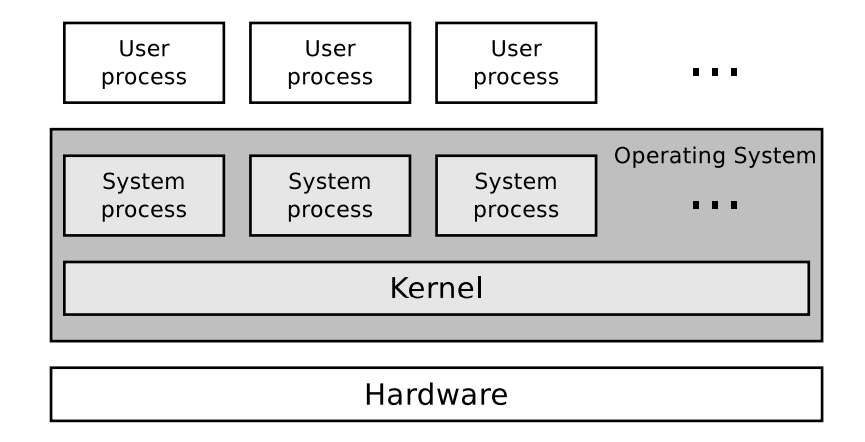
\includegraphics[width=.7\textwidth]{img/osStructure.png}
        
        \begin{itemize}
            \item \textbf{User Processes} process the user's jobs.
            \item \textbf{System Processes} provide services of the operating system
            \item \textbf{The operating system core} (Kernel) contains all components of the operating system, which are not implemented as system processes.
            
            %\item There are 4 types of Operating Systems
        \end{itemize}

        % Batch processing operating system
        \item \textbf{Batch processing} Operating Systems \\
        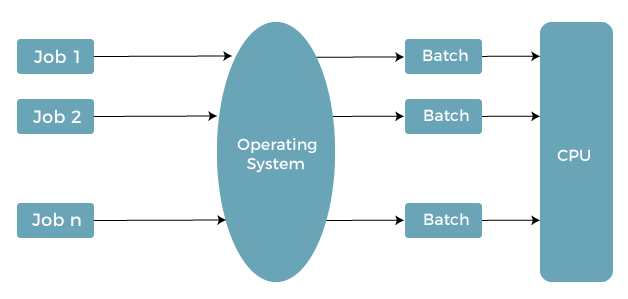
\includegraphics[width=.7\textwidth]{img/batch-operating-system1.png}
            \begin{itemize}
                \item Each program needs to be provided completely with all input data before the beginning of the execution.

                \item Batch processing is well suited for the execution of routine tasks.

                \item $\Rightarrow$ \textbf{Objective}: Maximize CPU utilization.
                
                \item $\Rightarrow$ \textbf{Drawback}: During I/O operations, the CPU is idle.
                
            \end{itemize}
        
        \underline{\textbf{z.B:}} non-interactive batch files and shell scripts.

        % Time-sharing operating systems
        \item \textbf{Time-sharing} (interactive mode) Operating Systems \\ 
        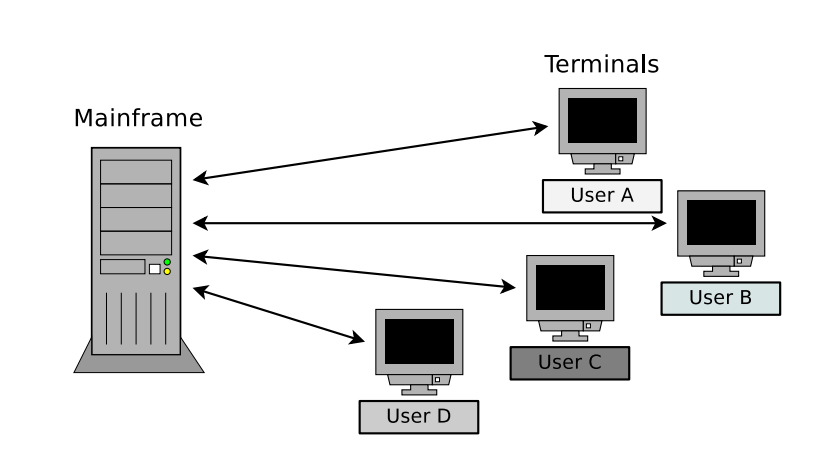
\includegraphics[width=.7\textwidth]{img/time-sharing.png}
        \begin{itemize}
            \item \textbf{Multiple users} work with a single computer in a simultaneous and competitive way sharing the available computing time of the CPU. \\
             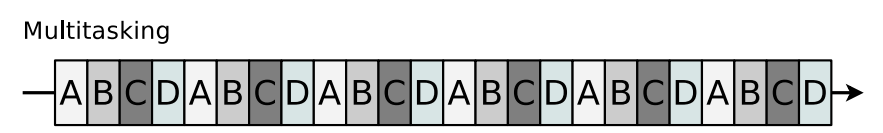
\includegraphics[width=.74\textwidth]{img/time-sharing-multitasking.png}

            \item $\Rightarrow$ \textbf{Objective}: Minimize the response time.
            
        \end{itemize}
        
        % Single-tasking
        \item \textbf{Single-tasking Operating Systems}
        \begin{itemize}
            \item At any given moment, only a single program is executed.
            
            \item Multiple started programs are executed one after other.
            
            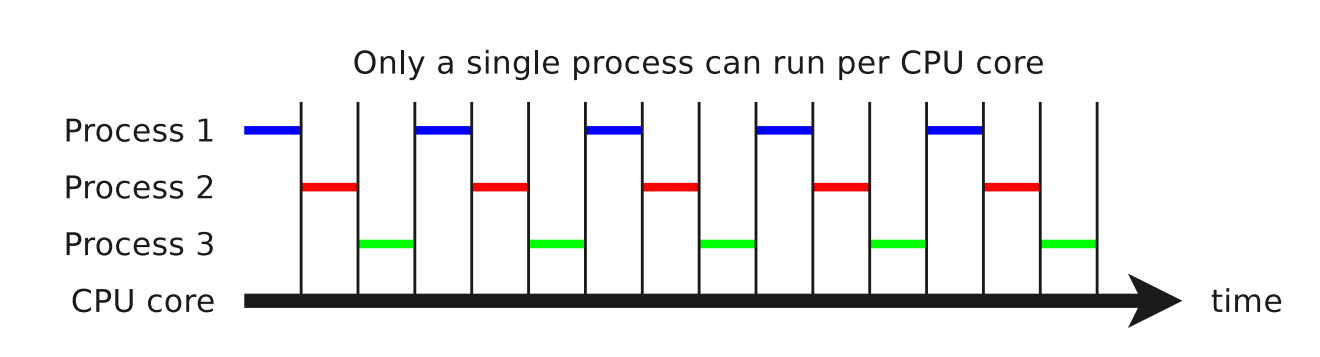
\includegraphics[width=.78\textwidth]{img/singletasking_CPU_time.png}
            
            \item 
            
        \end{itemize}
    
    
    	% multi-tasking operating systems
    	\item \textbf{Multi-tasking Operating systems}
    	\begin{itemize}
    		\item Multiple programs can be executed at the same time (with multiple CPUs/Cores) or quasi-parallel.
    		
    		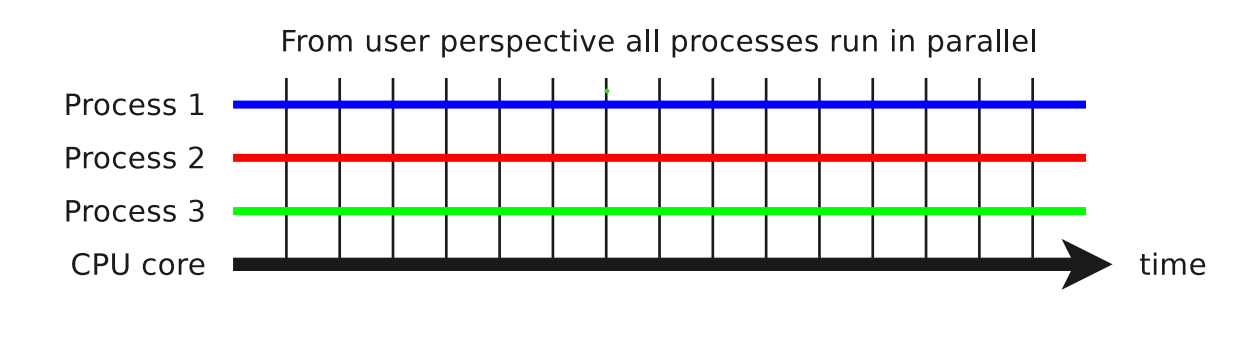
\includegraphics[width=.78\textwidth]{img/multitasking_CPU_time.png}
    		
    		\item
    	\end{itemize}
    
    
    	% Single-User vs Multi-User
    	\item \textbf{Single-User vs Multi-User}
    	\begin{itemize}
    		\item Single-User 
    	\end{itemize}
        
        
    \end{enumerate}


\section{Exam WS21.22}
Solutions:

\begin{itemize}
    \item Question 1
    \begin{enumerate}
        \item \colorbox{Aquamarine}{Kernel} is a computer program at the core of a computer's operating system and generally has complete control over everything in the system.
        
        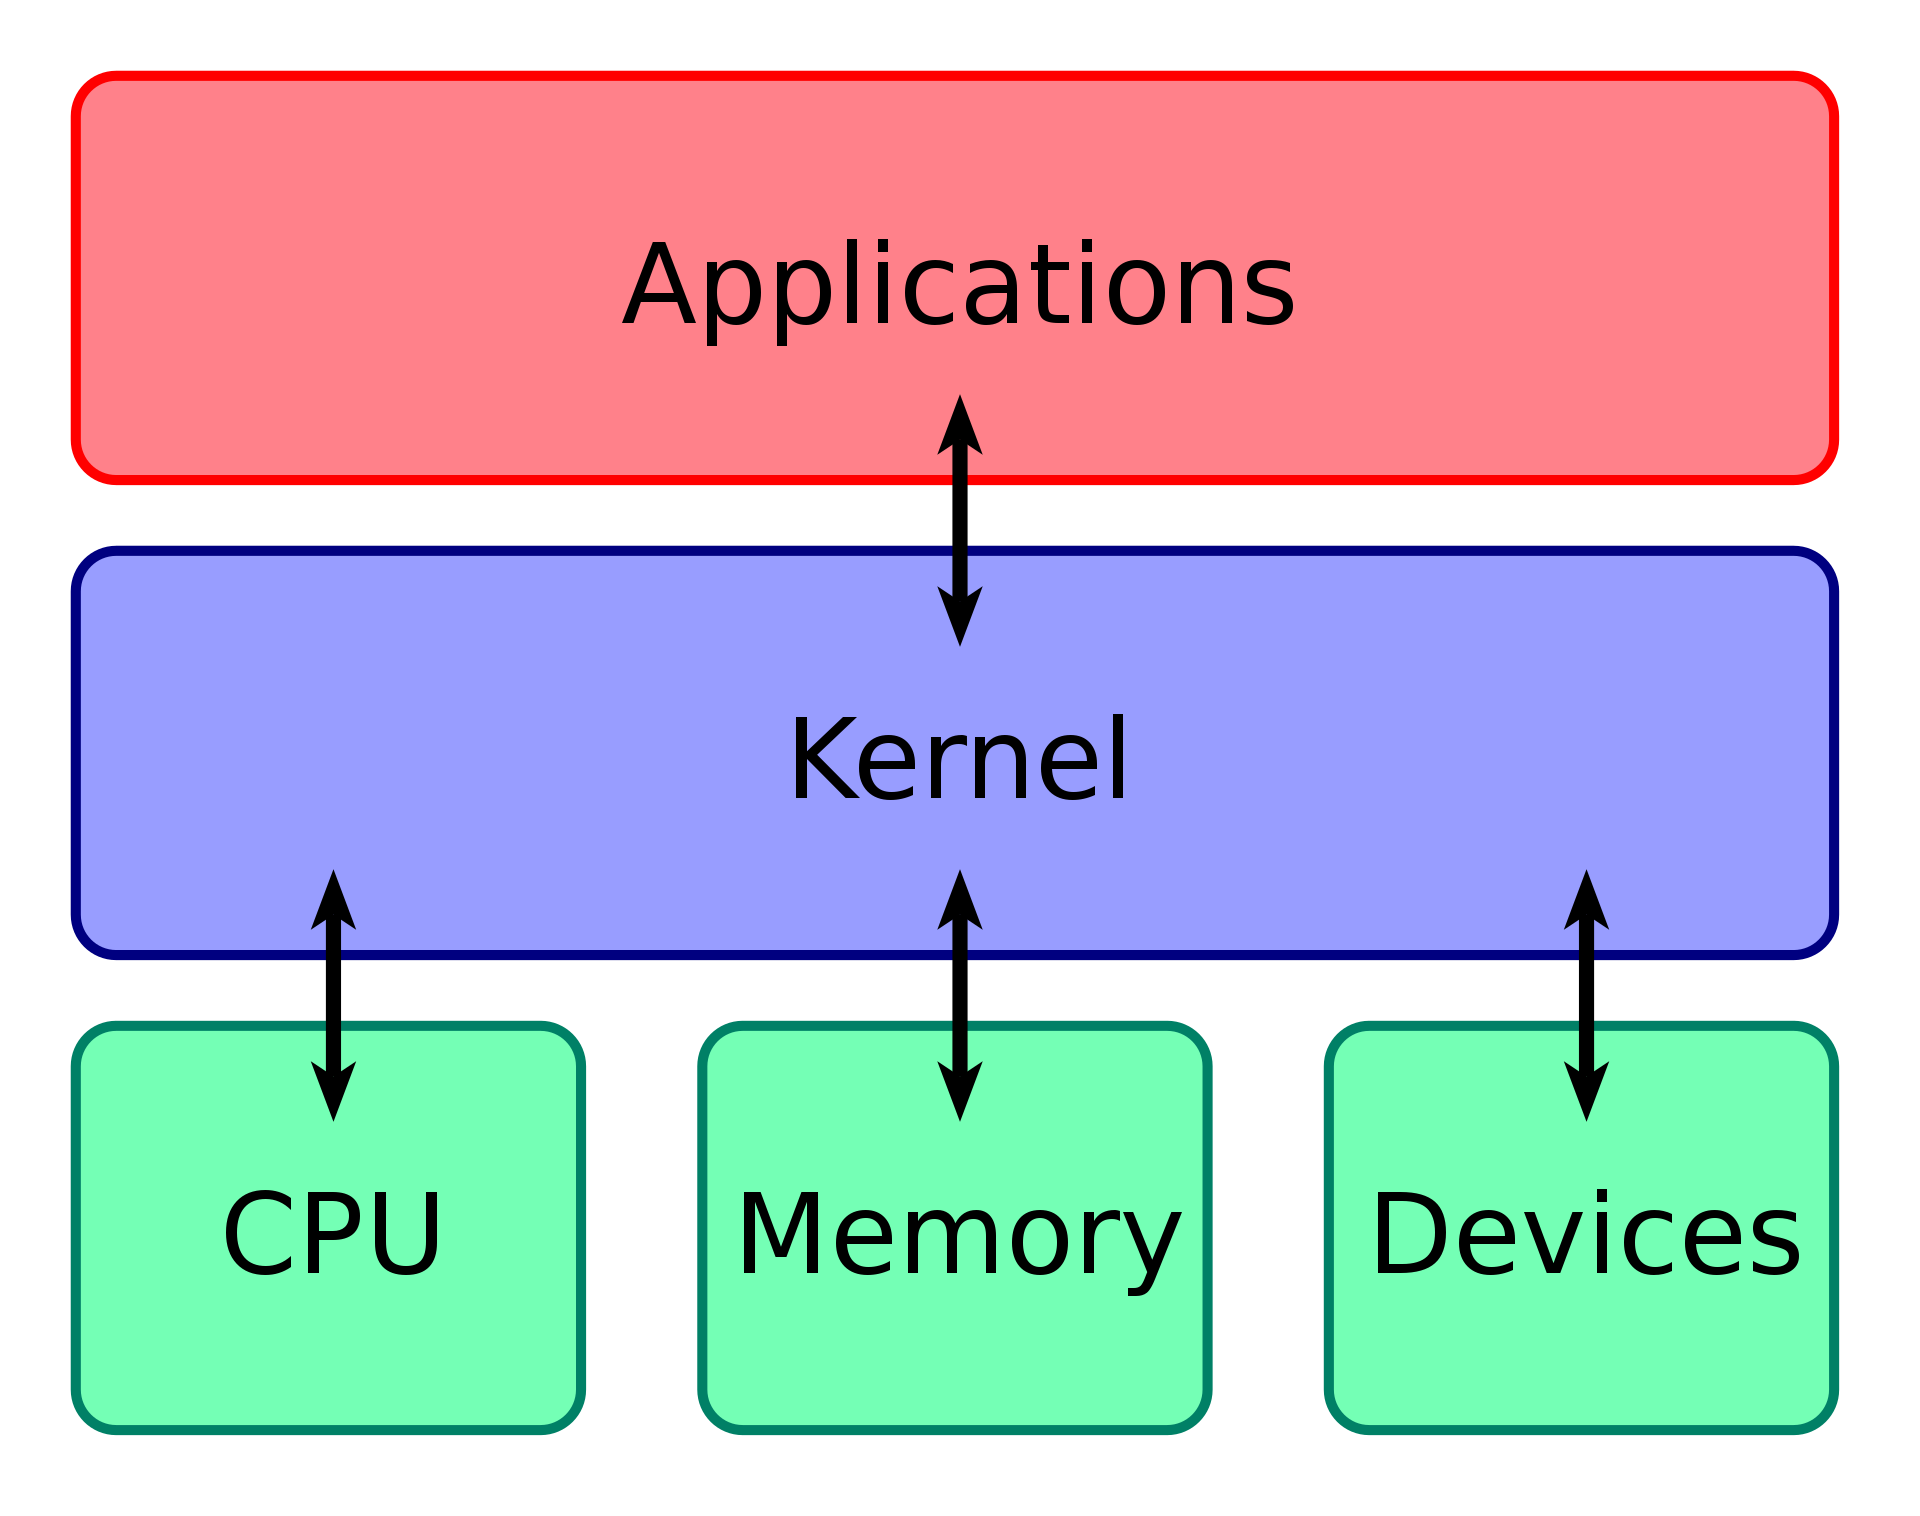
\includegraphics[width=.43\textwidth]{img/Kernel1.png}

        \item \colorbox{BurntOrange}{Monolithic Kernel}  is a type of \colorbox{Aquamarine}{Kernel} in which 

        
    \end{enumerate}
\end{itemize}

    

\end{document}
